%manuel 6e, chapitre G3
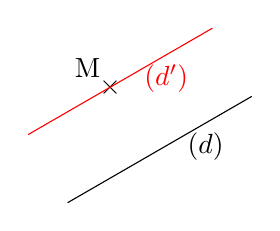
\begin{tikzpicture}[scale=.5,every node/.style={scale=1},rotate=30]

\draw (0,2) node [above left]{M};
\draw (0,2) node {$\times$};
\draw (-2.4,0)--(3,0) node [near end,below] {$(d)$};
\draw [red](-2.4,2)--(3,2) node [near end,below] {$(d')$};

\end{tikzpicture} 
